\chapter{Chapter One}
\section{Introduction}
Weather radar is an invaluable tool for nowcasting severe weather. In Canada, lake-effect snows are a severe weather event which have big impacts on a large
sector of the population. While the current Canadian C-Band radar systems have been proven in this regard, there is uncertainty with whats to come with the
new S-Band systems. While no prototype system is available to test in the Great Lakes area, the next best stand-in to compare with are the current S-Band
radars in the United States. King City radar (CWKR) has been compared with the Buffalo, NY radar (KBUF) previously by \cite{Boodoo2015}, but this case was
for rainfall. Furthermore, C-Band radars have been compared with S-band radars before by \cite{Abon2014}, but polarimetric variables weren't considered. To
compare the two radars, the data will be objectively analyzed. Radar data objective analysis is most prominently used in created mosaics of multiple radars
for projects such as the Multi-Radar Multi-Sensor project by NSSL \citep{Zhang2016}. It is also used extensively for research purposes, including studying
snow squalls \citep{Mulholland2017}.  The goal of this study is to show that there will be no loss in quality of radar observations for the purposes of
nowcasting lake-effect snow with S-Band radar. Another goal is to directly compare polarimetric moments, which has not been done in this manner before, and
identify any biases. It is important to remove biases as no amount of spatial or temporal smoothing will remove them. With bias-adjusted values from two independent sources, a high-confidence conclusion can be made on the types of hydrometeors present in the common sampling volumes. Although dual-pol radar has matured within the research community, operational deployment has been a much slower process. Many studies have been undertaken in regards to quantitative precipitation estimation using dual-pol variables for rainfall, but studies involving snow have been much more limited. Findings here should increase confidence in comparing dual-polarmetric at two different wavelengths, and demonstration the information rich nature of these variables. 
\section{Background}
First, it is important to provide some background on the weather radar moments that are presented in this study, from both single and dual polarized signals.
The convention for representing these moments symbolically hereafter is lower-case subscript for linear units and upper-case subscript for logarithmic units,
i.e. $Z_{DR}$ is logarithmic while $Z_{dr}$ is linear.
\subsection{Radar Locations}
In Canada, there is one active C-band weather radar with dual-pol capabilities. It is located north of Toronto, in King City, with rest of the network is
currently undergoing an upgrade to polarimetric S-Band. Its neighbor to the south, KBUF, was upgraded to dual-pol in 2012 as part of a network wide upgrade. 
\begin{figure}[h]
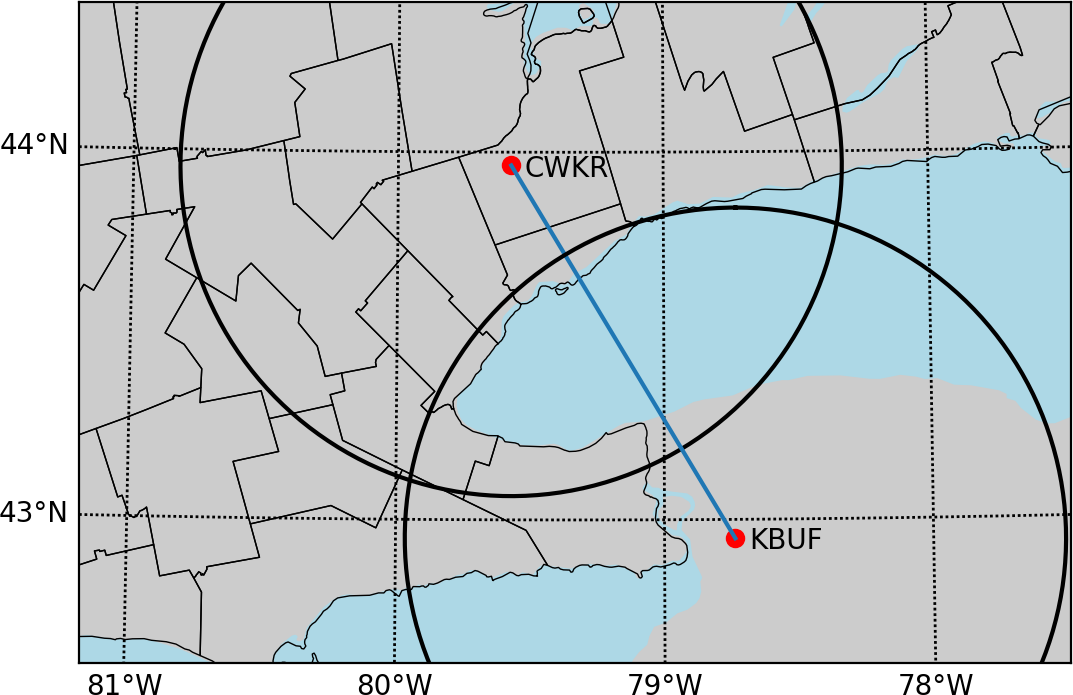
\includegraphics[width=\textwidth]{map}
\caption{The location of the NWS Buffalo Radar (KBUF) and King City Radar (CWKR) are shown as red dots, with a 100 km range ring around each. The distance
between the two, drawn as a blue line, is 131.5 km.} 
\label{map}
\end{figure}
Figure \ref{map} shows the geographic location of the radar sites in comparison with each other.
\subsection{Reflectivity Factor ($Z_{h}$)}
The foremost moment derived from radar is the reflectivity factor ($Z_{h}$), where the
subscript denotes its derivation from the horizontally polarized signal. This variable
measures the number density $N(D)$ of hydrometeors of diameter $D$ per unit volume, as
presented in Equation \ref{eq:ref_factor}. Due to uncertainties about what type of
target is actually doing the scattering, it is typically represented as the equivalent
reflectivity factor $Z_{eh}$, where $Z_{h}$ = $Z_{eh}$ if the targets are made of liquid 
water and are comparatively small to the wavelength \citep{Fabry2015}. The two names are 
essentially interchangeable, but the nomenclature $Z_{eh}$ will be used in this study to 
acknowledge the presence of non-ideal targets, e.g. snow crystals.
\begin{equation}\label{eq:ref_factor}
Z_{h} = \int_0^{\infty} N(D)D^6dD \ (mm^6/m^3)
\end{equation}
\subsection{Differential Reflectivity ($Z_{dr}$)}
Radars equipped with dual-polarimetric (dual-pol) capabilities are still an emerging technology, in terms of operational meteorological applications. These
types of radar systems are capable of transmitting and receiving two orthogonally polarized electromagnetic waves in order to deduce more information about
the microphysical structure of hydrometeors. One of the main variables this allows them to produce is $Z_{DR}$, defined as the ratio of the horizontal
channel reflectivity ($Z_H$) to the vertical channel reflectivity $Z_{V}$). This can be simplified to the difference between the two using the logarithmic
quotient rule, since they are represented in logarithmic units. Equation \ref{eq:zdr} demonstrates this concept.
\begin{equation}\label{eq:zdr}
Z_{dr} = 10 * \log_{10}(\frac{Z_H}{Z_V}) = Z_h - Z_v
\end{equation}
\subsubsection{Interpretations of $Z_{DR}$ in Snow}
In snowfall, $Z_{DR}$ can be a powerful tool for deducing the predominant crystal habit and type. Values of $Z_{DR}$ typically observed for dry aggregated snow at cold temperatures range from $0 < Z_{DR} < 0.2$ dB, while pristine ice crystals and lightly aggregated crystals range from $0.4 < Z_{DR} < 3$ dB, both for a range of $Z_{eH}$ of $5 < Z_{eH} < 30$ dBZ. Figure \ref{zdr_chart} shows expected $Z_{DR}$ for frozen and liquid hydrometeors, as well as non-meteorological targets. In this study, we are only concerned with hydrometeors that are sufficiently frozen.
\begin{figure}[H]
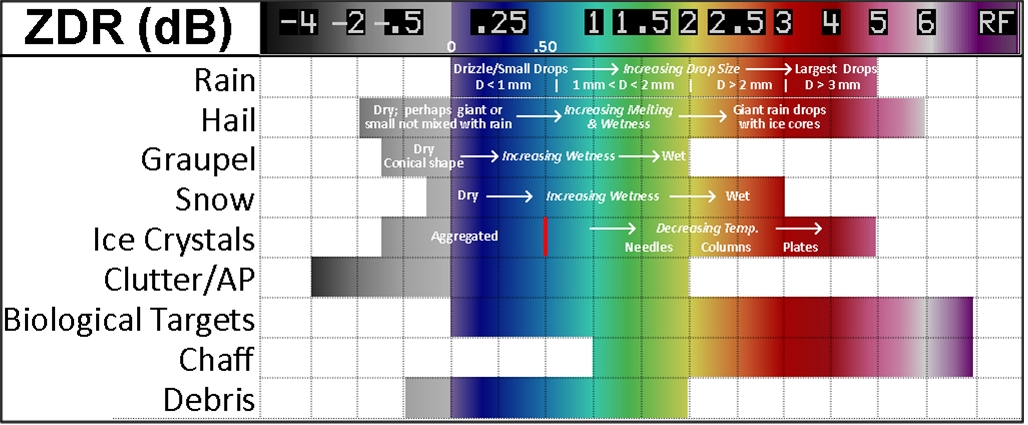
\includegraphics[width=\textwidth]{zdr_chart}
\caption{Chart of expected ranges of $Z_{DR}$ for a variety of targets. Taken from \citet{Fabry2015}.} 
\label{zdr_chart}
\end{figure}
\subsection{Co-polar Cross-Correlation Coefficient ($\rho_{hv}$)}
With the advent of Simultaneous Transmit and Receive (STAR) radar systems, which both radars used here have, it is possible to perform the zero time-lag
cross-correlation between the time series data obtained from horizontal and vertical channels. This is known as the Co-polar Cross-Correlation Coefficient
($\rho_{hv}$) in radar meteorology, and ranges from 0 to 1. Low values indicate pulse volumes containing heterogeneities, while a value of 1 indicates
matching, homogenous volumes. For an ensemble of scatters, Equation \ref{eq:backscatter} defines the backscattering matrix used in the definition of
$\rho_{hv}$ in Equation \ref{eq:rhohv}, as defined by \citet{Ryzhkov2007b}.
\begin{equation}\label{eq:backscatter}
\mathbf{S} = \begin{bmatrix}
             S_{hh}       & S_{hv} \\
             S_{hv}       & S_{vv} \\
             \end{bmatrix}
\end{equation}
\begin{equation}\label{eq:rhohv}
\rho_{hv} = \frac{\langle{S_{vv}{S_{hh}}^{*}\rangle}}{\sqrt{\langle{{S_{hh}}^{2}\rangle}\langle{{S_{vv}}^{2}\rangle}}}
\end{equation}
\subsubsection{Interpretations of $\rho_{hv}$ in Snow}
Contamination from clutter and other non-meteorological targets can be achieved by using a $\rho_{hv}$ threshold of 0.95, as suggested by \citet{Straka2000}.
Using this threshold can also be used to avoid non-Rayleigh scatters, which becomes a bigger problem at C-Band wavelengths \citet{Fabry2015}.
 



